\author{Benjamin Besic}
Der Anfang der Planung war die Besprechung des alten Programms und was an dem nicht passt bzw. verbessert gehört.

\section{Use Cases}

\subsection{Kantinenarbeiter}

\begin{compactitem}
    \item Neue Menüs anlegen
    \begin{compactitem}
        \item Ein Kantinenmitarbeiter kann für jeden Tag neue Menüs mit drei Hauptspeisen und deren Kategorien, einer Vorspeise und einer Nachspeise anlegen.
    \end{compactitem}
    \item Vorhandene Menüs editieren
    \begin{compactitem}
        \item Die Bezeichnungen der bereits erstellten Menüs sollen verändert werden können.
    \end{compactitem}
    \item Übersicht der täglichen Bestellungen
    \begin{compactitem}
        \item Die Kantinenmitarbeiter sollen eine Übersicht, der an einem bestimmten Tag bestellten Menüs haben. Diese inkludiert die zusammengefasste Bestellanzahl der verschiedenen Menüs und eine Liste von allen Bestellungen.
    \end{compactitem}
    \item Bestellungsübersicht drucken
    \begin{compactitem}
        \item Die Übersicht wie vorher beschrieben soll zu einem PDF-Objekt konvertiert werden und dementsprechend ausgedruckt werden können.
    \end{compactitem}
\end{compactitem}

\subsection{Mitarbeiter}

\begin{compactitem}
    \item Menüs bestellen
    \begin{compactitem}
        \item Ein Mitarbeiter hat eine Auswahl aller Menüs und kann für jeden Tag eine der drei Hauptspeisen auswählen. Nach der Auswahl kann er die Essenszeit auswählen, die Anzahl und nötige Kommentare hinzufügen.
    \end{compactitem}
    \item Menüs für andere Mitarbeiter bestellen
    \begin{compactitem}
        \item Ein Mitarbeiter kann den obrigen Bestellvorgang für einen anderen Mitarbeiter ausführen. 
    \end{compactitem}
    \item Übersicht aller Bestellungen
    \begin{compactitem}
        \item Als Mitarbeiter soll man alle seine vergangenen Bestellungen und deren Informationen in einer Übersicht einsehen können. Diese Übersicht kann filtriert werden.
    \end{compactitem}
    \item Bestellungen stornieren
    \begin{compactitem}
        \item In der oben genannten Übersicht soll man die Möglichkeit haben eine Bestellung auszuwählen und zu stornieren, wenn dies möglich ist.
    \end{compactitem}
    \item Bestellstatistiken einsehen
    \begin{compactitem}
        \item Ein Mitarbeiter soll Diagramme zur Verfügung haben, wo er sein Bestellverhalten einsehen kann.
    \end{compactitem}
\end{compactitem}
\pagebreak


\section{Datenmodell-Diagramme}
Der nächste Arbeitsschritt war die Entwicklung eines Datenmodells, welches die Basis der Programmlogik sein soll. Dieses wurde mittels ERD-Diagramm erstellt.
\begin{figure}[htp]
    \centering
    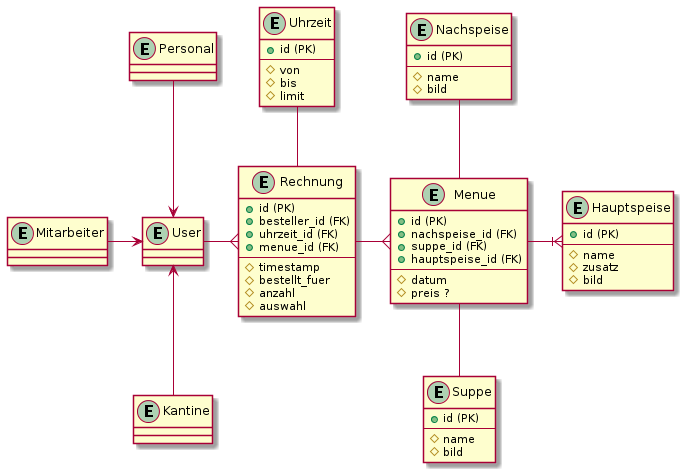
\includegraphics[scale=0.5]{pics/erd-alt.png}
    \caption{Erste Version des Datenmodells}
    \label{fig:impl:ERDold}
\end{figure}

\begin{figure}[htp]
    \centering
    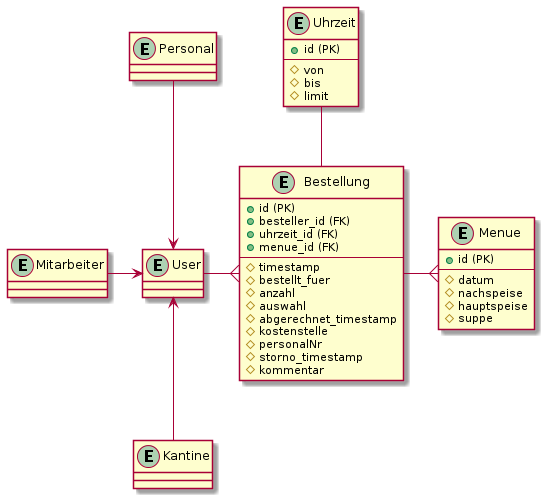
\includegraphics[scale=0.5]{pics/erd-aktuell.png}
    \caption{Finale Version des Datenmodells}
    \label{fig:impl:ERDold}
\end{figure}
\pagebreak

\section{UI entwickeln}

Nachdem das Datenmodell feststand wurden UI-Prototypen entwickelt, die das Aussehen der Vue-App darstellen sollen.

\begin{figure}[htp]
    \author{Benjamin Besic}
    \centering
    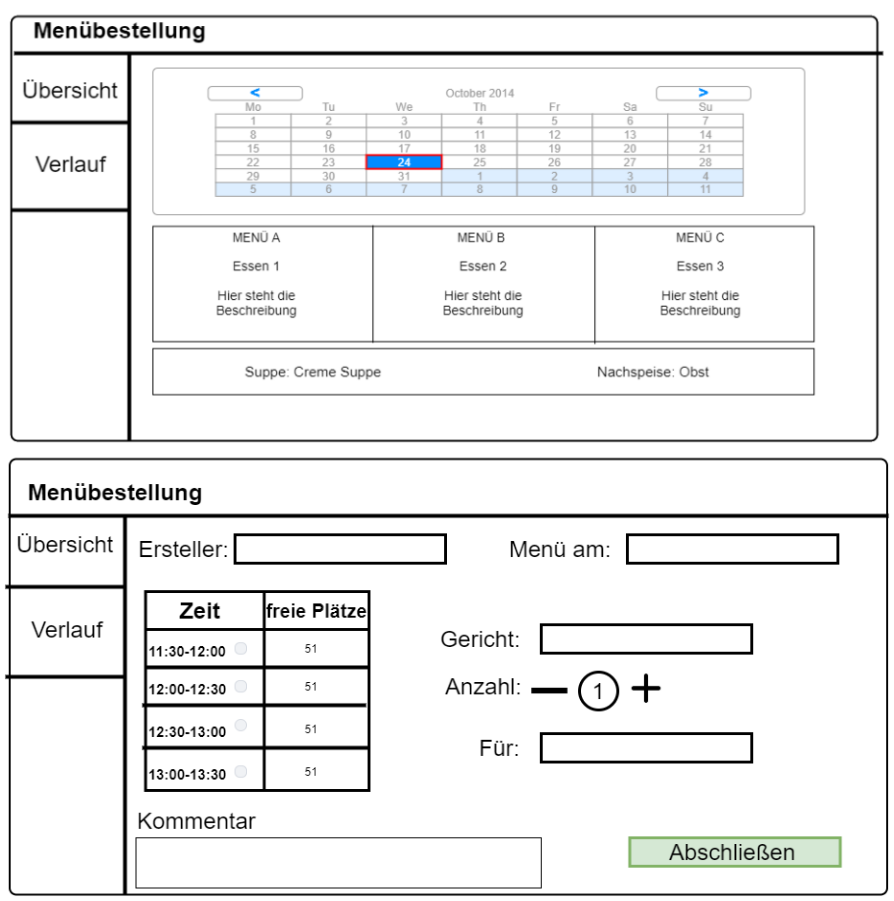
\includegraphics[scale=0.36]{pics/UI-Bestellung-Prototyp.png}
    \caption{UI-Prototypen für den Bestellvorgang}
    \label{fig:impl:UIPlanningBest}
\end{figure}

\begin{figure}[htp]
    \author{Benjamin Besic}
    \centering
    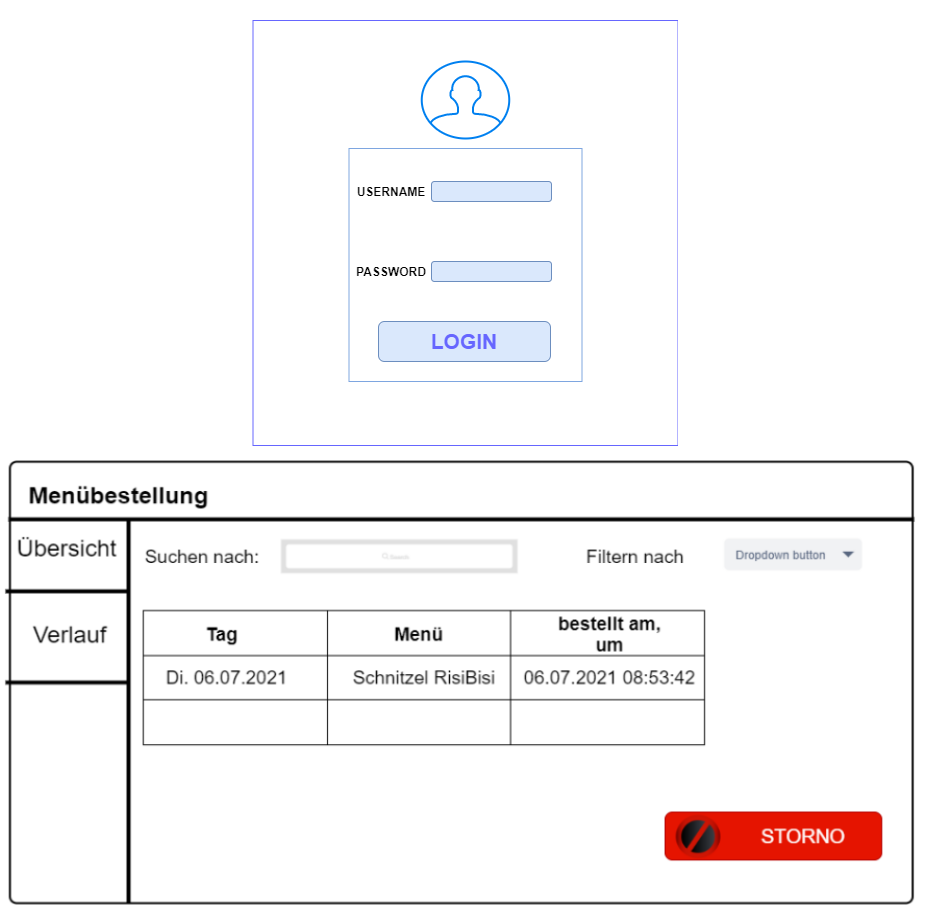
\includegraphics[scale=0.36]{pics/UI-Login-Uebersicht-Prototyp.png}
    \caption{UI-Prototypen für den den Login und die Übersicht}
    \label{fig:impl:UIPlanningLogUebersicht}
\end{figure}

\pagebreak

\section{Technologien}
Beim Entwickeln wurden folgende Technologien verwendet:
\begin{itemize}
    \item docker 3.1
    \item Vue.js 2.6.14
    \item quarkus 2.5.0.Final
    \item Jetpack Compose 1.0.1
    \item Keycloak 14.0.0
    \item Java OpenJDK-11
    \item Java EE 8
    \item JBoss Wildfly 7.3.4.GA
\end{itemize}